\newsavebox{\PreviewAppGraphic}
\begingroup
\makeatletter
\let\PreviewEndFloatBox\@endfloatbox
\def\@endfloatbox{\PreviewEndFloatBox
\typeout{FONE-FLOAT-HEIGHT=\the\ht\@currbox}
\typeout{FONE-FLOAT-DEPTH=\the\dp\@currbox}}
\makeatother
\begin{figure*}[t]
  \centering
  \sbox{\PreviewAppGraphic}{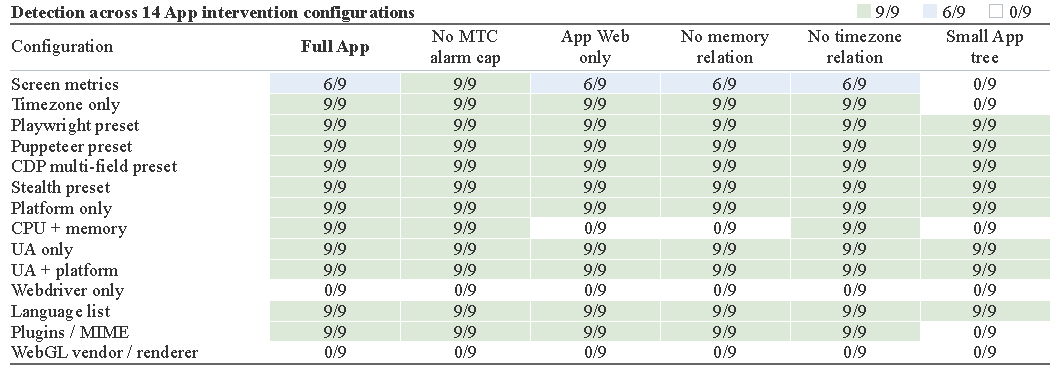
\includegraphics[width=\textwidth]{figures/F01_main_rev4.pdf}}
\typeout{FONE-TEXTWIDTH=\the\textwidth}
\typeout{FONE-COLUMNWIDTH=\the\columnwidth}
\typeout{FONE-TEXTHEIGHT=\the\textheight}
\typeout{FONE-GRAPHIC-WIDTH=\the\wd\PreviewAppGraphic}
\typeout{FONE-GRAPHIC-HEIGHT=\the\ht\PreviewAppGraphic}
\typeout{FONE-GRAPHIC-DEPTH=\the\dp\PreviewAppGraphic}
\usebox{\PreviewAppGraphic}
  \caption{Saved detection results for 14 App modification configurations and six methods. Cells show T/N with N=9 per row; green, blue and unfilled cells denote 9/9, 6/9 and 0/9. Totals over the 14 configurations are reported separately. Full App excludes standalone-browser C1 and unintegrated Host/resource conditions. Removing the MTC alarm cap cannot be judged superior here; normal-record costs are reported separately. These materials have a development-use history and are not a new experiment or blind test.}
  \Description{Fourteen modification configurations in the original order and six App methods. Every cell shows the saved alarm count out of nine. Pale green denotes full detection, pale blue denotes partial detection, and zero-detection cells have no fill; a compact three-swatch legend shares the title row. The numbers carry all values. Zero detections and partial detections remain explicit.}
  \label{fig:app-modification-detection}
\end{figure*}
\endgroup
